%
% kruemmung.tex -- Kruemmungsradius
%
% (c) 2017 Prof Dr Andreas Müller, Hochschule Rapperswil
%
\documentclass[tikz]{standalone}
\usepackage{times}
\usepackage{txfonts}
\usepackage{pgfplots}
\usepackage{csvsimple}
\usetikzlibrary{arrows,intersections}
\begin{document}
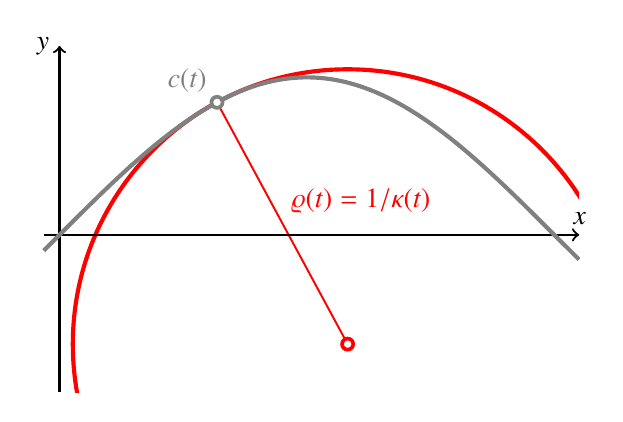
\begin{tikzpicture}[thick,scale=2]
\coordinate (O) at (0,0);

\draw[red,line width=0.7] (1.00000, 0.84147)--(1.82954,-0.69385);
\draw[red,fill=blue]  (1.82954,-0.69385) circle[radius=0.04] {};
\draw[red,fill=white] (1.82954,-0.69385) circle[radius=0.032] {};

\begin{scope}
\clip (0,-1) rectangle (3.3,1.2);
\draw[red,line width=1.5] (1.82954,-0.69385) circle[radius=1.7451];
\end{scope}

\draw[->] (-0.1,0)--(3.3,0) coordinate[label={above:$x$}];
\draw[->] (0,-1.0)--(0,1.2) coordinate[label={left:$y$}];

\draw[gray,domain=-0.1:3.3,line width=1.5,samples=100] plot (\x,{sin(180 * \x/3.14159)});

%\draw[->,gray,line width=1.5]
%(1,{sin(180 * 1 / 3.14159)})--(2,{sin(180 * 1 / 3.14159)+cos(180 * 1 / 3.14159)});

\draw[gray,fill=red] (1,{sin(180 * 1 / 3.14159)}) circle[radius=0.04] {};
\draw[gray,fill=white] (1,{sin(180 * 1 / 3.14159)}) circle[radius=0.032] {};

\node at (1,{sin(180 * 1 / 3.14159)}) [above left,gray] {$c(t)$};
%\node at (1+0.8,{sin(180 * 1 / 3.14159)+0.8*cos(180 * 1 / 3.14159)}) [above left,gray] {$\dot c(t)$};

%    1.00000    1.00000    0.84147    1.00000    0.54030    0.87979    0.47535    0.00000   -0.84147    0.47535   -0.87979   -0.57304    1.82954   -0.69385

\node at (2.82/2, 0.147/2) [above right,red] {$\varrho(t)=1/\kappa(t)$};

\end{tikzpicture}
\end{document}


